% Created by tikzDevice version 0.10.1 on 2017-09-04 19:52:36
% !TEX encoding = UTF-8 Unicode
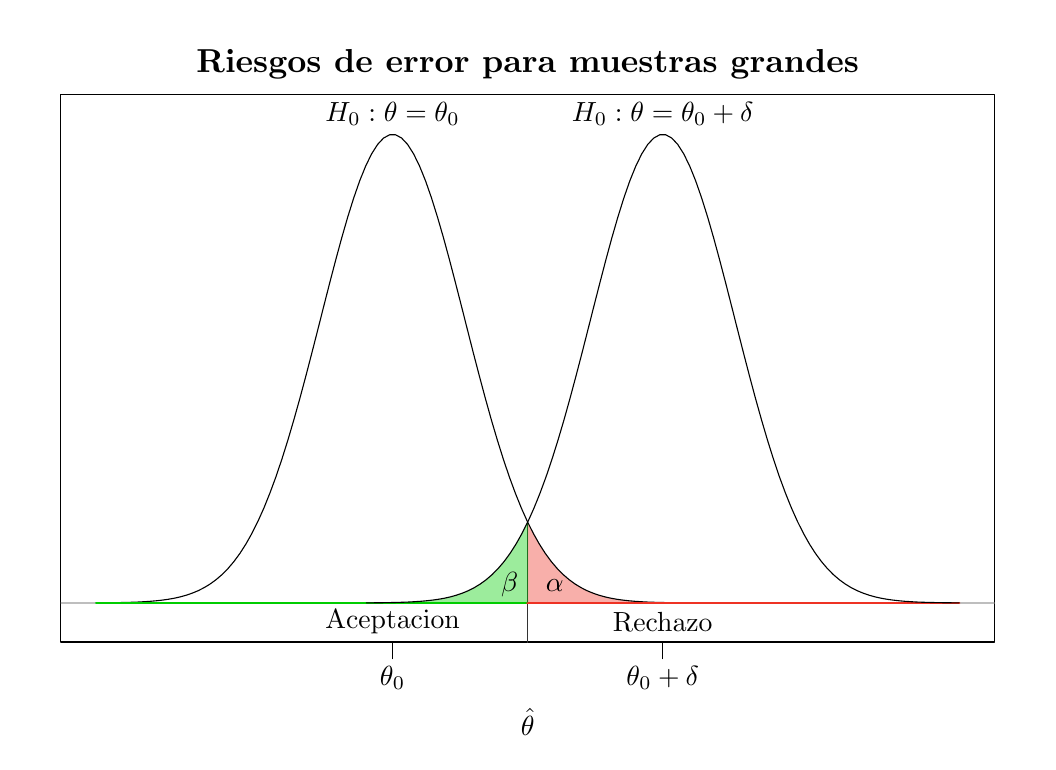
\begin{tikzpicture}[x=1pt,y=1pt]
\definecolor{fillColor}{RGB}{255,255,255}
\path[use as bounding box,fill=fillColor,fill opacity=0.00] (0,0) rectangle (361.35,258.00);
\begin{scope}
\path[clip] (  0.00,  0.00) rectangle (361.35,258.00);
\definecolor{drawColor}{RGB}{0,0,0}

\path[draw=drawColor,line width= 0.4pt,line join=round,line cap=round] ( 12.00, 36.00) --
	(349.35, 36.00) --
	(349.35,234.00) --
	( 12.00,234.00) --
	( 12.00, 36.00);
\end{scope}
\begin{scope}
\path[clip] (  0.00,  0.00) rectangle (361.35,258.00);
\definecolor{drawColor}{RGB}{0,0,0}

\node[text=drawColor,anchor=base,inner sep=0pt, outer sep=0pt, scale=  1.20] at (180.67,241.86) {\bfseries Riesgos de error para muestras grandes};

\node[text=drawColor,anchor=base,inner sep=0pt, outer sep=0pt, scale=  1.00] at (180.67,  2.40) {$\hat\theta$};
\end{scope}
\begin{scope}
\path[clip] ( 12.00, 36.00) rectangle (349.35,234.00);
\definecolor{drawColor}{RGB}{190,190,190}

\path[draw=drawColor,line width= 0.4pt,line join=round,line cap=round] ( 12.00, 50.12) -- (349.35, 50.12);
\definecolor{fillColor}{RGB}{238,50,36}

\path[fill=fillColor,fill opacity=0.39] (180.54, 50.12) --
	(180.54, 79.60) --
	(182.71, 75.27) --
	(184.87, 71.43) --
	(187.03, 68.05) --
	(189.19, 65.10) --
	(191.36, 62.55) --
	(193.52, 60.37) --
	(195.68, 58.51) --
	(197.85, 56.94) --
	(200.01, 55.63) --
	(202.17, 54.53) --
	(204.34, 53.64) --
	(206.50, 52.90) --
	(208.66, 52.30) --
	(210.83, 51.82) --
	(212.99, 51.44) --
	(215.15, 51.14) --
	(217.32, 50.90) --
	(219.48, 50.71) --
	(221.64, 50.57) --
	(223.81, 50.45) --
	(225.97, 50.37) --
	(228.13, 50.31) --
	(230.30, 50.26) --
	(232.46, 50.22) --
	(234.62, 50.19) --
	(236.79, 50.17) --
	(238.95, 50.16) --
	(238.95, 50.12) --
	cycle;
\definecolor{drawColor}{gray}{0.20}

\path[draw=drawColor,line width= 0.4pt,line join=round,line cap=round] (180.54, 16.17) -- (180.54, 79.60);
\definecolor{drawColor}{RGB}{0,0,0}

\node[text=drawColor,anchor=base,inner sep=0pt, outer sep=0pt, scale=  1.00] at (190.44, 54.41) {$\alpha$};

\path[draw=drawColor,line width= 0.4pt,line join=round,line cap=round] ( 24.79, 50.16) --
	( 26.95, 50.17) --
	( 29.11, 50.19) --
	( 31.28, 50.22) --
	( 33.44, 50.26) --
	( 35.60, 50.31) --
	( 37.77, 50.37) --
	( 39.93, 50.45) --
	( 42.09, 50.57) --
	( 44.26, 50.71) --
	( 46.42, 50.90) --
	( 48.58, 51.14) --
	( 50.75, 51.44) --
	( 52.91, 51.82) --
	( 55.07, 52.30) --
	( 57.24, 52.90) --
	( 59.40, 53.64) --
	( 61.56, 54.53) --
	( 63.73, 55.63) --
	( 65.89, 56.94) --
	( 68.05, 58.51) --
	( 70.22, 60.37) --
	( 72.38, 62.55) --
	( 74.54, 65.10) --
	( 76.71, 68.05) --
	( 78.87, 71.43) --
	( 81.03, 75.27) --
	( 83.20, 79.60) --
	( 85.36, 84.43) --
	( 87.52, 89.79) --
	( 89.69, 95.66) --
	( 91.85,102.05) --
	( 94.01,108.92) --
	( 96.17,116.25) --
	( 98.34,123.98) --
	(100.50,132.04) --
	(102.66,140.35) --
	(104.83,148.83) --
	(106.99,157.36) --
	(109.15,165.82) --
	(111.32,174.10) --
	(113.48,182.05) --
	(115.64,189.54) --
	(117.81,196.45) --
	(119.97,202.64) --
	(122.13,208.00) --
	(124.30,212.42) --
	(126.46,215.82) --
	(128.62,218.12) --
	(130.79,219.29) --
	(132.95,219.29) --
	(135.11,218.12) --
	(137.28,215.82) --
	(139.44,212.42) --
	(141.60,208.00) --
	(143.77,202.64) --
	(145.93,196.45) --
	(148.09,189.54) --
	(150.26,182.05) --
	(152.42,174.10) --
	(154.58,165.82) --
	(156.75,157.36) --
	(158.91,148.83) --
	(161.07,140.35) --
	(163.24,132.04) --
	(165.40,123.98) --
	(167.56,116.25) --
	(169.73,108.92) --
	(171.89,102.05) --
	(174.05, 95.66) --
	(176.22, 89.79) --
	(178.38, 84.43) --
	(180.54, 79.60) --
	(182.71, 75.27) --
	(184.87, 71.43) --
	(187.03, 68.05) --
	(189.19, 65.10) --
	(191.36, 62.55) --
	(193.52, 60.37) --
	(195.68, 58.51) --
	(197.85, 56.94) --
	(200.01, 55.63) --
	(202.17, 54.53) --
	(204.34, 53.64) --
	(206.50, 52.90) --
	(208.66, 52.30) --
	(210.83, 51.82) --
	(212.99, 51.44) --
	(215.15, 51.14) --
	(217.32, 50.90) --
	(219.48, 50.71) --
	(221.64, 50.57) --
	(223.81, 50.45) --
	(225.97, 50.37) --
	(228.13, 50.31) --
	(230.30, 50.26) --
	(232.46, 50.22) --
	(234.62, 50.19) --
	(236.79, 50.17) --
	(238.95, 50.16);

\node[text=drawColor,anchor=base,inner sep=0pt, outer sep=0pt, scale=  1.00] at (131.87,224.17) {$H_0: \theta = \theta_0$};
\end{scope}
\begin{scope}
\path[clip] (  0.00,  0.00) rectangle (361.35,258.00);
\definecolor{drawColor}{RGB}{0,0,0}

\path[draw=drawColor,line width= 0.4pt,line join=round,line cap=round] (131.87, 36.00) -- (131.87, 36.00);

\path[draw=drawColor,line width= 0.4pt,line join=round,line cap=round] (131.87, 36.00) -- (131.87, 30.00);

\node[text=drawColor,anchor=base,inner sep=0pt, outer sep=0pt, scale=  1.00] at (131.87, 20.40) {$\theta_0$};
\end{scope}
\begin{scope}
\path[clip] ( 12.00, 36.00) rectangle (349.35,234.00);
\definecolor{drawColor}{RGB}{0,205,0}

\path[draw=drawColor,line width= 1.0pt,line join=round,line cap=round] ( 24.79, 50.12) -- (180.54, 50.12);
\definecolor{drawColor}{RGB}{238,50,36}

\path[draw=drawColor,line width= 1.0pt,line join=round,line cap=round] (336.56, 50.12) -- (180.54, 50.12);
\definecolor{drawColor}{RGB}{0,0,0}

\node[text=drawColor,anchor=base,inner sep=0pt, outer sep=0pt, scale=  1.00] at (131.87, 40.86) {Aceptacion};

\node[text=drawColor,anchor=base,inner sep=0pt, outer sep=0pt, scale=  1.00] at (229.48, 39.89) {Rechazo};
\definecolor{fillColor}{RGB}{0,205,0}

\path[fill=fillColor,fill opacity=0.39] (122.40, 50.12) --
	(122.40, 50.16) --
	(124.56, 50.17) --
	(126.73, 50.19) --
	(128.89, 50.22) --
	(131.05, 50.26) --
	(133.22, 50.31) --
	(135.38, 50.37) --
	(137.54, 50.45) --
	(139.71, 50.57) --
	(141.87, 50.71) --
	(144.03, 50.90) --
	(146.20, 51.14) --
	(148.36, 51.44) --
	(150.52, 51.82) --
	(152.69, 52.30) --
	(154.85, 52.90) --
	(157.01, 53.64) --
	(159.18, 54.53) --
	(161.34, 55.63) --
	(163.50, 56.94) --
	(165.67, 58.51) --
	(167.83, 60.37) --
	(169.99, 62.55) --
	(172.16, 65.10) --
	(174.32, 68.05) --
	(176.48, 71.43) --
	(178.64, 75.27) --
	(180.81, 79.60) --
	(180.81, 50.12) --
	cycle;

\node[text=drawColor,anchor=base,inner sep=0pt, outer sep=0pt, scale=  1.00] at (174.17, 54.41) {$\beta$};

\path[draw=drawColor,line width= 0.4pt,line join=round,line cap=round] (122.40, 50.16) --
	(124.56, 50.17) --
	(126.73, 50.19) --
	(128.89, 50.22) --
	(131.05, 50.26) --
	(133.22, 50.31) --
	(135.38, 50.37) --
	(137.54, 50.45) --
	(139.71, 50.57) --
	(141.87, 50.71) --
	(144.03, 50.90) --
	(146.20, 51.14) --
	(148.36, 51.44) --
	(150.52, 51.82) --
	(152.69, 52.30) --
	(154.85, 52.90) --
	(157.01, 53.64) --
	(159.18, 54.53) --
	(161.34, 55.63) --
	(163.50, 56.94) --
	(165.67, 58.51) --
	(167.83, 60.37) --
	(169.99, 62.55) --
	(172.16, 65.10) --
	(174.32, 68.05) --
	(176.48, 71.43) --
	(178.64, 75.27) --
	(180.81, 79.60) --
	(182.97, 84.43) --
	(185.13, 89.79) --
	(187.30, 95.66) --
	(189.46,102.05) --
	(191.62,108.92) --
	(193.79,116.25) --
	(195.95,123.98) --
	(198.11,132.04) --
	(200.28,140.35) --
	(202.44,148.83) --
	(204.60,157.36) --
	(206.77,165.82) --
	(208.93,174.10) --
	(211.09,182.05) --
	(213.26,189.54) --
	(215.42,196.45) --
	(217.58,202.64) --
	(219.75,208.00) --
	(221.91,212.42) --
	(224.07,215.82) --
	(226.24,218.12) --
	(228.40,219.29) --
	(230.56,219.29) --
	(232.73,218.12) --
	(234.89,215.82) --
	(237.05,212.42) --
	(239.22,208.00) --
	(241.38,202.64) --
	(243.54,196.45) --
	(245.71,189.54) --
	(247.87,182.05) --
	(250.03,174.10) --
	(252.20,165.82) --
	(254.36,157.36) --
	(256.52,148.83) --
	(258.69,140.35) --
	(260.85,132.04) --
	(263.01,123.98) --
	(265.18,116.25) --
	(267.34,108.92) --
	(269.50,102.05) --
	(271.66, 95.66) --
	(273.83, 89.79) --
	(275.99, 84.43) --
	(278.15, 79.60) --
	(280.32, 75.27) --
	(282.48, 71.43) --
	(284.64, 68.05) --
	(286.81, 65.10) --
	(288.97, 62.55) --
	(291.13, 60.37) --
	(293.30, 58.51) --
	(295.46, 56.94) --
	(297.62, 55.63) --
	(299.79, 54.53) --
	(301.95, 53.64) --
	(304.11, 52.90) --
	(306.28, 52.30) --
	(308.44, 51.82) --
	(310.60, 51.44) --
	(312.77, 51.14) --
	(314.93, 50.90) --
	(317.09, 50.71) --
	(319.26, 50.57) --
	(321.42, 50.45) --
	(323.58, 50.37) --
	(325.75, 50.31) --
	(327.91, 50.26) --
	(330.07, 50.22) --
	(332.24, 50.19) --
	(334.40, 50.17) --
	(336.56, 50.16);
\end{scope}
\begin{scope}
\path[clip] (  0.00,  0.00) rectangle (361.35,258.00);
\definecolor{drawColor}{RGB}{0,0,0}

\path[draw=drawColor,line width= 0.4pt,line join=round,line cap=round] (229.48, 36.00) -- (229.48, 36.00);

\path[draw=drawColor,line width= 0.4pt,line join=round,line cap=round] (229.48, 36.00) -- (229.48, 30.00);

\node[text=drawColor,anchor=base,inner sep=0pt, outer sep=0pt, scale=  1.00] at (229.48, 20.40) {$\theta_0+\delta$};
\end{scope}
\begin{scope}
\path[clip] ( 12.00, 36.00) rectangle (349.35,234.00);
\definecolor{drawColor}{RGB}{0,0,0}

\node[text=drawColor,anchor=base,inner sep=0pt, outer sep=0pt, scale=  1.00] at (229.48,224.17) {$H_0: \theta = \theta_0 + \delta$};
\end{scope}
\end{tikzpicture}
